\documentclass[border=10pt]{standalone}

\usepackage{tikz}
\usepackage{tikzsymbols}
\usetikzlibrary{calc,patterns,shapes.geometric}

\def\centerarc[#1](#2)(#3:#4:#5){\draw[#1] ($(#2)+({#5*cos(#3)},{#5*sin(#3)})$) arc (#3:#4:#5);}

\begin{document}
	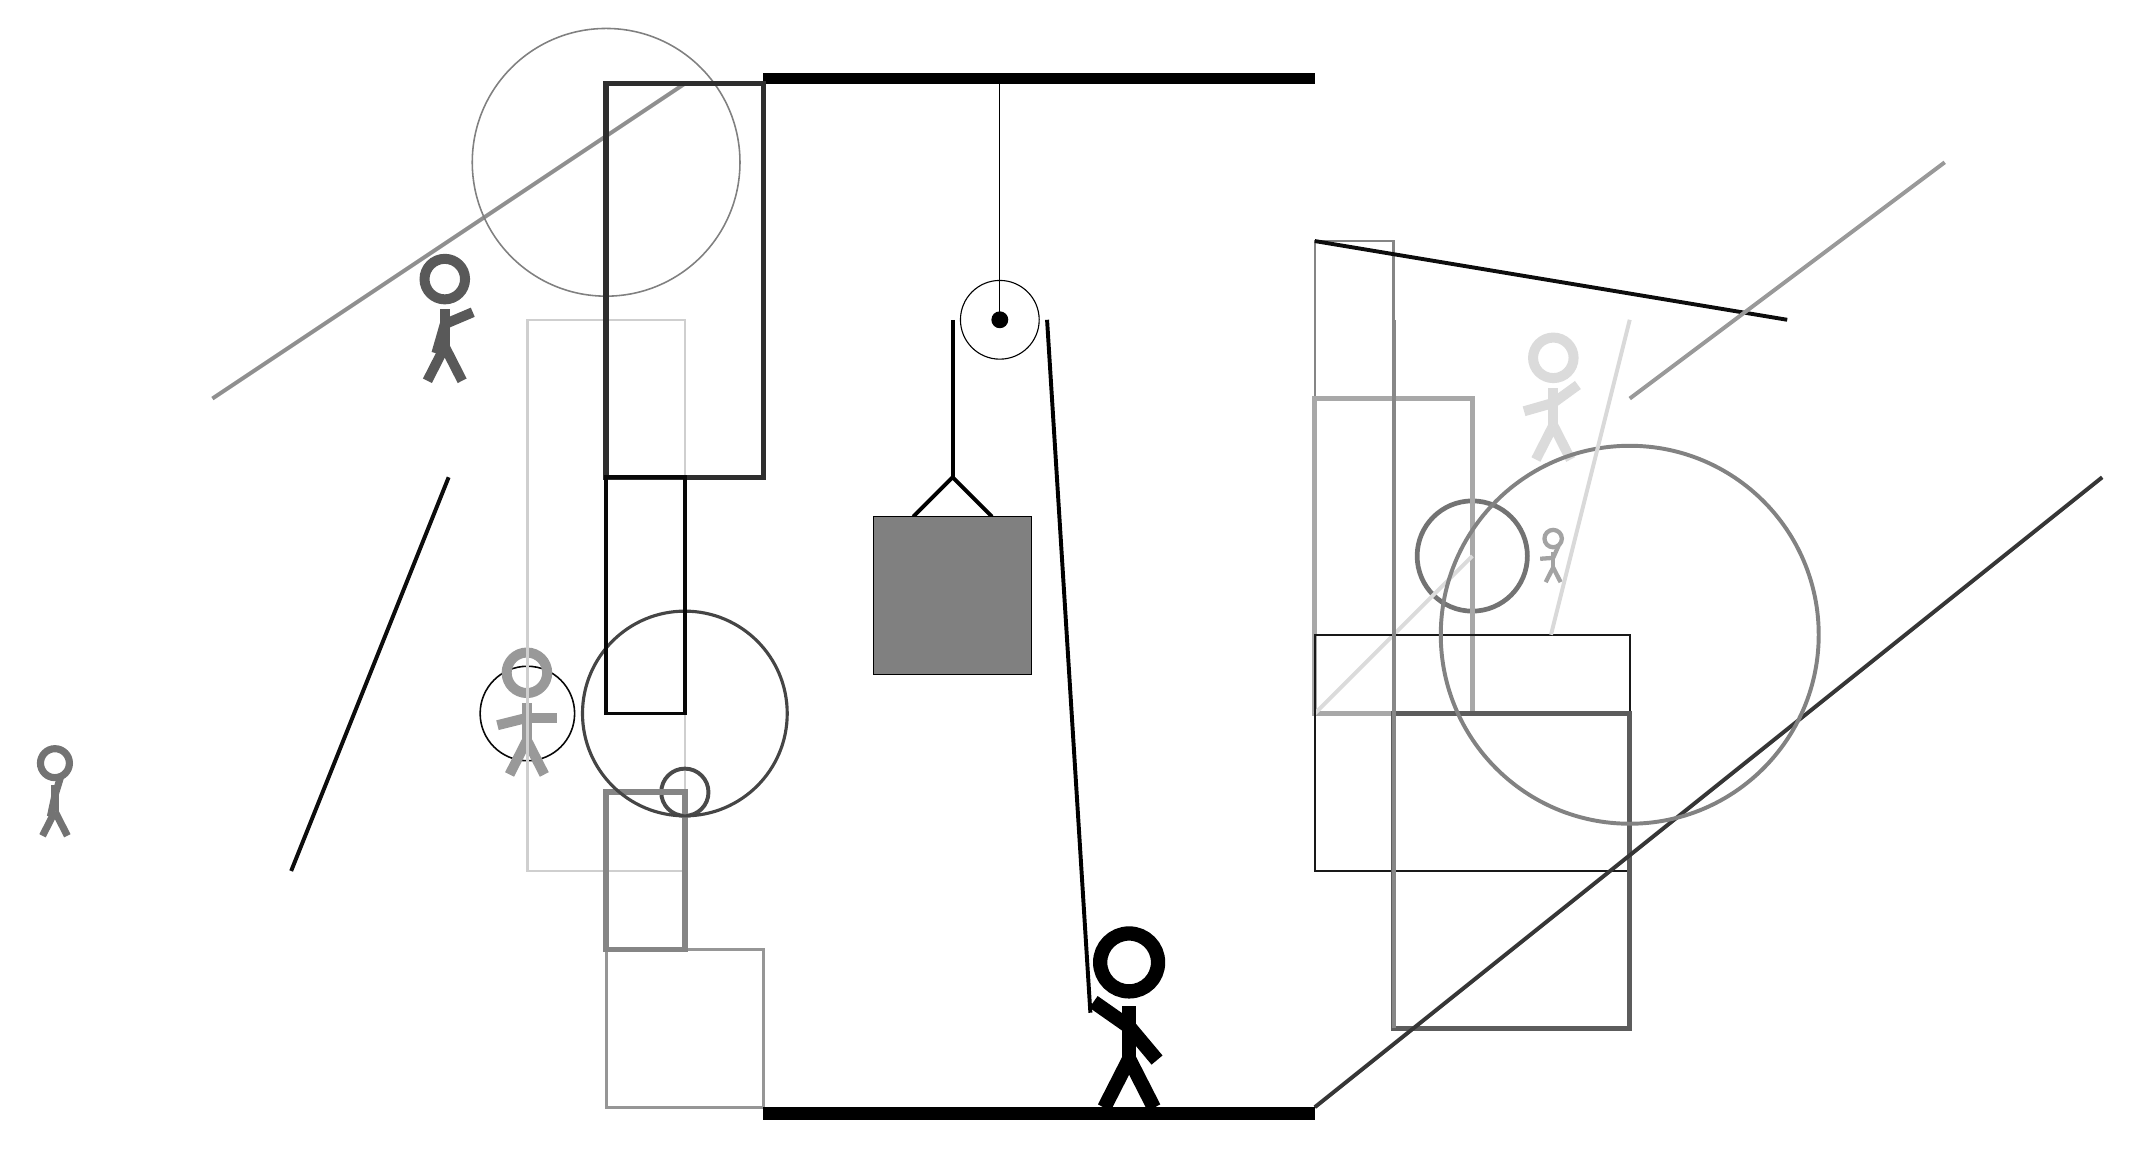
\begin{tikzpicture}
		%%%%% START %%%%%
		
		\draw[fill=black] (-2, 10) rectangle (5, 10.125);
		
		\draw (1, 7) circle (0.5);
		\draw[fill=black] (1, 7) circle (0.1);
		\draw (1, 10) -- (1, 7);
		
		\draw[line width=0.5mm] (-0.1, 4.5) -- (0.4, 5.0) -- (0.9, 4.5);
		\draw[fill=black!50] (-0.6, 4.5) rectangle (1.4, 2.5);
		
		\draw [line width=0.6mm, color=black!55](7, 4) circle (0.7);
		
		\node[line width=0.4mm, color=black!65] at (-6, 7) {\Strichmaxerl[7][74][23]};
		\draw[line width=0.4mm, color=black!41] (-2, -3) rectangle (-4, -1);
		\draw[line width=0.3mm, color=black!48] (6, 3) rectangle (5, 8);
		\draw[line width=0.5mm, color=black!95](-6, 5) -- (-8, 0);
		\node[line width=0.4mm, color=black!36] at (8, 4) {\Strichmaxerl[3][4][66]};
		\draw[line width=0.6mm, color=black!34] (7, 6) rectangle (5, 2);
		\draw[line width=0.5mm, color=black!14](5, 2) -- (7, 4);
		\draw[line width=0.2mm, color=black!90] (5, 3) rectangle (9, 0);
		\draw [line width=0.2mm, color=black!97](-5, 2) circle (0.6);
		
		\node[line width=0.6mm, color=black!40] at (-5, 2) {\Strichmaxerl[7][14][0]};
		\draw[line width=0.5mm, color=black!95](5, 8) -- (11, 7);
		\draw[line width=0.3mm, color=black!19] (-3, 0) rectangle (-5, 7);
		\draw [line width=0.5mm, color=black!71](-3, 1) circle (0.3);
		\draw[line width=0.5mm, color=black!40](9, 6) -- (13, 9);
		\node[line width=0.3mm, color=black!55] at (-11, 1) {\Strichmaxerl[5][78][73]};
		\draw[line width=0.6mm, color=black!64] (6, -2) rectangle (9, 2);
		
		\draw[line width=0.5mm, color=black!79](5, -3) -- (15, 5);
		\draw[line width=0.7mm, color=black!48] (-4, -1) rectangle (-3, 1);
		
		\node[line width=0.4mm, color=black!14] at (8, 6) {\Strichmaxerl[7][16][36]};
		\draw[line width=0.5mm, color=black!44](-3, 10) -- (-9, 6);
		
		\draw [line width=0.4mm, color=black!73](-3, 2) circle (1.3);
		\draw [line width=0.2mm, color=black!50](-4, 9) circle (1.7);
		\draw[line width=0.5mm, color=black!47](6, -2) -- (6, 7);
		\draw[line width=0.7mm, color=black!82] (-2, 5) rectangle (-4, 10);
		
		\draw [line width=0.5mm, color=black!49](9, 3) circle (2.4);
		
		\draw[line width=0.5mm, color=black!97] (-4, 5) rectangle (-3, 2);
		\draw[line width=0.5mm, color=black!15](9, 7) -- (8, 3);
		
		\draw[line width=0.5mm] (0.4, 7) -- (0.4, 5.0);
		\centerarc[line width=0.5mm](1, 7)(0:180:0.6);
		\draw[line width=0.5mm](1.6, 7) -- (2.15, -1.8);
		
		\node at (2.6, -1.9) {\Strichmaxerl[10][-35][-50]};
		
		\draw[fill=black] (-2, -3) rectangle (5, -3.15);
		
		%%%%% END %%%%%
	\end{tikzpicture}
\end{document}